\subsection{Мотивация работы}

\begin{frame}
    \frametitle{Постановка магистерской работы}
    \centering
    \begin{itemize}
        \item Сложность задания $d$, знания учащегося $u$
        \item Модель Эло $$
            p(x=1|d,u) = \frac{1}{1+\exp(d-u)}
        $$
        \item Адаптивные алгоритмы задают оптимальный уровень попыток $s^*$ на
        исход выполнения задания 
    \end{itemize}
    \begin{block}{Алгоритм Роббинса-Монро}
        Пускай $x$ - бернулевская случайная величина с параметром $s=f(d)$, где $f(x)$ - выпуклая.
        Тогда для cхема пересчета $d_t=\mathbf{x}_t + a_t (s^* - x_t)$ с шагами $a_t$ удовлетворяющих условиям
        $\sum_{t=0}^{\infty} a_t = \infty, \sum_{t=0}^{\infty} a_t^2 < \infty$,
        выполняет cпуск к целевому значению $\lim_{t \rightarrow \infty} d_t = d^*$, где $d^* : s(d^*) = s^*$.
    \end{block}
\end{frame}



\begin{frame}
  \centering \Large
  \emph{Постановка для диссертации}
\end{frame}


\begin{frame}
    \frametitle{Индивидуальное обучение}
    \centering

    \begin{figure}
        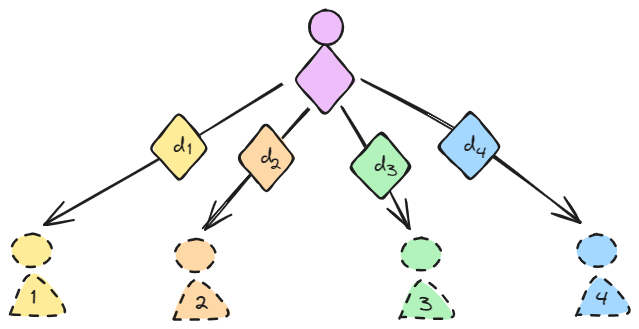
\includegraphics[width=0.9\linewidth]{assets/setting/ideal.excalidraw.png}
    \end{figure} 
\end{frame}

\begin{frame}
    \begin{block}{Постановка}
        Каждый учащийся $i$ получает задачу сложности $d_i$, соответствующую текущему развитию
    \end{block}

    \begin{exampleblock}{Преимущества}
        \begin{itemize}
            \item адаптивное обучение
            \item сроки исполнения выбираются из потребностей обучающегося
        \end{itemize}

    \end{exampleblock}

    \begin{alertblock}{Недостатки}
        \begin{itemize}
            \item проверка большого числа заданий
            \item координация работы
        \end{itemize}
    \end{alertblock}
\end{frame}


\begin{frame}
    \frametitle{Коллективное обучение}
    \centering
    \begin{figure}
        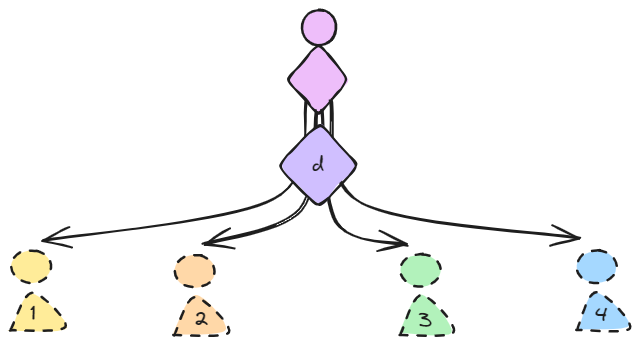
\includegraphics[width=0.9\linewidth]{assets/setting/real.excalidraw.png}
    \end{figure} 
\end{frame}

\begin{frame}
    \begin{block}{Постановка}
        Все обучающиеся выполняют одну задачу сложности $d$
    \end{block}
    \begin{exampleblock}{Преимущества}
        \begin{itemize}
            \item возможность предварительной подготовки программы
            \item поощряет соревновательный дух
            \item относительная простота проверки
        \end{itemize}
    \end{exampleblock}
    \begin{alertblock}{Проблемы}
        \begin{itemize}
            \item отсутствие интереса у отстающих и одаренных обучающихся
            \item сложность учета индивидуальных потребностей
        \end{itemize}
    \end{alertblock}
\end{frame}


\begin{frame}
    \frametitle{Постановка для кандидатской диссертации}
    \centering
    \begin{block}{Цель}
        Определение оптимальных стратегий обучений в группах с использованием адаптивных алгоритмов сложности
    \end{block}

    \begin{block}{Задачи}
        \begin{itemize}
            \item демонстрация несостоятельности базового алгоритма Роббинса-Монро для коллективного обучения
            \item изучение распределения нагрузки между учащимися с учетом супераддитивности функций совместной работы
            \item разработка алгоритма адаптивной сложности для работы с группами
        \end{itemize}
    \end{block}

\end{frame}

